%%%%%%%%%%%%%%%%%%%%%%%%%%%%
% CHAPTER                  %
%%%%%%%%%%%%%%%%%%%%%%%%%%%%
\chapter{Chapter One}%
\label{chap:chapter_one}

%%%%%%%%%%%%%%%%%%%%%%%%%%%%
% SECTION                  %
%%%%%%%%%%%%%%%%%%%%%%%%%%%%
\section{Section One}
\label{chap:section_one}

  %%%%%%%%%%%%%%%%%%%%%%%%%%%%
  % SUBSECTION               %
  %%%%%%%%%%%%%%%%%%%%%%%%%%%%
  \subsection{Sub section One}

  And your chapter one goes here\cite{web001}\@. ~\\
  Lorem ipsum dolor sit amet, consectetur adipisicing elit, sed do eiusmod
  tempor incididunt ut labore et dolore magna aliqua. Ut enim ad minim veniam,
  quis nostrud exercitation ullamco laboris nisi ut aliquip ex ea commodo
  consequat. Duis aute irure dolor in reprehenderit in voluptate velit esse
  cillum dolore eu fugiat nulla pariatur. Excepteur sint occaecat cupidatat non
  proident, sunt in culpa qui officia deserunt mollit anim id est laborum.

  \begin{figure}[H]%
    \center%
    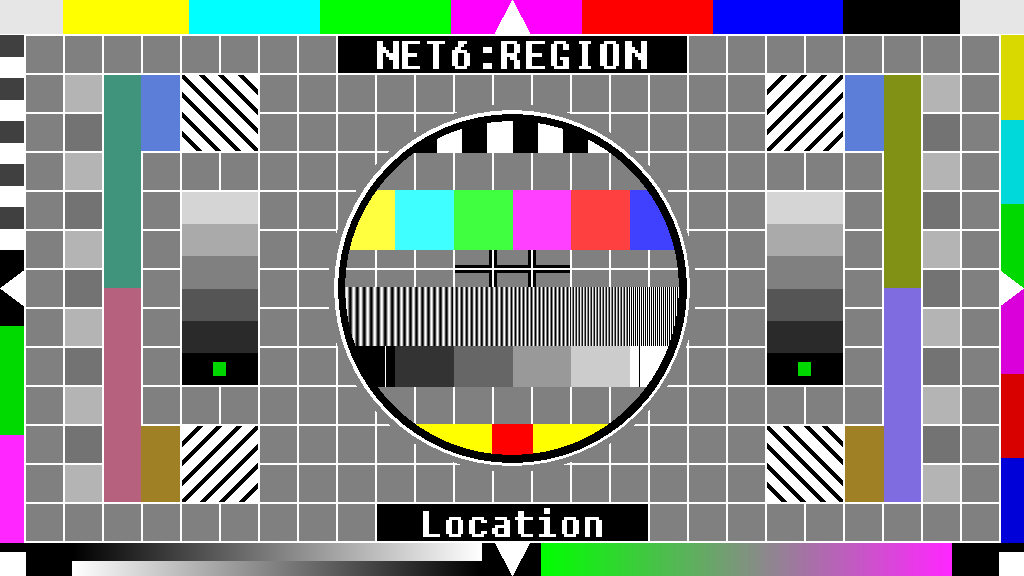
\includegraphics[width=0.3\textwidth]{test.png}%
    \caption[This is a test image]{Test Image}\label{fig:test}%
  \end{figure}
  
   \begin{figure}[H]%
    \center%
    
\includegraphics[width=0.3\textwidth]{garbage.png}%
    \caption[This is a test image]{garbage Image}\label{fig:test}%
  \end{figure}

  %%%%%%%%%%%%%%%%%%%%%%%%%%%%
  % SUBSECTION               %
  %%%%%%%%%%%%%%%%%%%%%%%%%%%%
  \subsection{Sub section Two}

  This is a second subsection\cite{bazerman1988shaping}. ~\\
  Lorem ipsum dolor sit amet, consectetur adipisicing elit, sed do eiusmod
  tempor incididunt ut labore et dolore magna aliqua. Ut enim ad minim veniam,
  quis nostrud exercitation ullamco laboris nisi ut aliquip ex ea commodo
  consequat. Duis aute irure dolor in reprehenderit in voluptate velit esse
  cillum dolore eu fugiat nulla pariatur. Excepteur sint occaecat cupidatat non
  proident, sunt in culpa qui officia deserunt mollit anim id est laborum.

  \begin{description}\addtolength{\itemsep}{-0.35\baselineskip}%
  
    \item[\textbullet~\bfseries Menu Item] \hfill \\%
      Menu Description.~\\%
      {\textbf{Focus topics:~}\emph{Topic one, topic two, topic three, ...}}%
    %
    
    \item[\textbullet~\bfseries Menu Item] \hfill \\%
      Menu Description.~\\% 
      {\textbf{Focus topics:~}\emph{Topic one, topic two, topic three, ...}}%
    
    % emph to emphasize
    %
    
    \item[\textbullet~\bfseries Menu Item] \hfill \\%
      Menu Description.~\\%
      {\textbf{Focus topics:~}\emph{Topic one, topic two, topic three, ...}}%
  
  \end{description}
  Also bullets such as:%
  \begin{itemize}\addtolength{\itemsep}{-0.35\baselineskip}%
    \item One%
        \begin{itemize}\addtolength{\itemsep}{-0.35\baselineskip}%
        \item sub One%
        \item sub Two%
        \item \ldots%
        \end{itemize}%
    \item Two%
    \item Three%
    \item Four%
    \item \ldots%
  \end{itemize}%
  
  
  order list
  \begin{enumerate}
      \item a
      \item b
       sub-list
            \begin{enumerate}
              \item x
              \item y
              \item z
            \end{enumerate}
      \item c
  \end{enumerate}
  
  

  %
\textbf{Example equation by komy} In physics, the mass-energy equivalence is stated 
by the equation $E=mc^2$, discovered in 1905 by Albert Einstein.\\
\textit{Example equation by komy} In physics, the mass-energy equivalence is stated 
\texttt{www.github.com \textbackslash our ptoject}
by the equation $$E=mc^2$$, discovered in 1905 by Albert Einstein.\\
Welcome to \Ac{ENIS}.~\\
Again, welcome to \Ac{ENIS}. ~\\
Your introduction goes here. ~\\

\textsc{Amira Yousif Mohamed ELBaradei}.\\

$$\left\{\frac{x_3}{x^2}\right\}$$
$$\left[\frac{x_3}{x^2}\right]$$
$$\left.\frac{d y}{d x}\right]_{x=0}$$

this will be auto numbered by latex according to division and subdiv
\begin{equation}
L' = {L}{\sqrt{1-\frac{v^2}{c^2}}}
\end{equation}



table example\\
\begin{center}

\begin{tabular}{ |p{3cm}||p{3cm}|p{3cm}|p{3cm}|  }
 \hline
 \multicolumn{4}{|c|}{Country List} \\
 \hline
 
 Country Name     or Area Name& ISO ALPHA 2 Code &ISO ALPHA 3 Code&ISO numeric Code\\
 \hline
 Afghanistan   & AF    &AFG&   004\\
 Aland Islands&   AX  & ALA   &248\\
 Albania &AL & ALB&  008\\
 Algeria    &DZ & DZA&  012\\
 American Samoa&   AS  & ASM&016\\
 Andorra& AD  & AND   &020\\
 Angola& AO  & AGO&024\\
 \hline
\end{tabular}

\end{center}
And for more chaptes, just copy the file ``004-chapter1.tex'' and edit the content, and then you'll have to add it to ``001-report.tex''.
%%%%%%%%%%%%%%%%%%%%%%%%%%%%%%%%%%%%%%%%%%%%%%%%%%%%%%%%%%%%%%%%%%%%%%%%%%%%%%%%%%%%%%%%%%%%%%%%%%%%%%%%%%%%%%%%%%